\section{Numerical validation}\label{sec:numerical-validation}

We compare the one-point BA construction ($N=1$) with independent integration of
Hamilton's equations on a genus-two hyperelliptic curve and a smooth
genus-three trigonal curve. Analytic BA values and derivatives use
Generapy's reference-normalized BA jets; directional sigma jets supply
the pair-mode potentials \cite{Generapy}. Periods and first- and
second-kind lifts are computed once per example, with fixed reference
normalizations. The canonical vector field is
then evaluated separately from the polynomial Hamiltonian
\cref{eq:BA-H0-flat}.

\subsection{Curves and prescribed BA data}

The hyperelliptic example uses
\begin{equation}\label{eq:numeric-hyperelliptic-curve}
 y^2=4x(x^2-1)(x^2-4),\qquad L=M=2,
\end{equation}
and hence has eight canonical mode pairs. The ordered point
abscissae are $0.1,2.3,0.5,3.0$, with positive real ordinates in the
first group and negative ordinates in the second. We use the Baker
differentials of \cref{eq:BA-curve,eq:BA-second-kind} and reference
vector $z_0=\omega e_2+\tfrac{4i}{5}(1,1)^{\trans}$, where
$\omega$ is the first-kind half-period matrix. These are the normalized
BA points $\widehat Q_k$ of \cref{eq:BA-general-dictionary}.
This choice gives real phase coefficients, positive normalized weights
and the all-positive real form
$\bar\xi_k=\xi_k^*$, $1\leq k\leq K$, and
$\bar\xi_{ij}=\xi_{ij}^*$, $1\leq i\leq L<j\leq K$.
Thus every mode power is a squared modulus on this explosive-type solution.

The trigonal example uses
\begin{equation}\label{eq:numeric-trigonal-curve}
 y^3=x^4+2x^3+3x^2+5x+7,\qquad L=M=3,
\end{equation}
and hence has fifteen canonical mode pairs. The compatible
first- and second-kind bases are
\begin{equation}\label{eq:numeric-trigonal-bases}
 du=\frac{(1,x,y)^{\trans}}{3y^2}\,dx,\qquad
 dr=\frac{((5x^2+6x+3)y,\,2xy,\,x^2)^{\trans}}{3y^2}\,dx.
\end{equation}
At the unique point at infinity write $x=s^{-3}$ and
$y=s^{-4}w(s)$, where
$w(s)^3=1+2s^3+3s^6+5s^9+7s^{12}$ and $w(0)=1$.
Let $\epsilon_3=e^{2\pi i/3}$. The points have $x=r^3$ and
$y=\epsilon_3^j f(r^3)^{1/3}$, where $f(x)$ is the quartic in
\cref{eq:numeric-trigonal-curve}, its displayed cube root is positive,
and the ordered $(r,j)$ lists are
\[
 (0.6,0),\ (0.9,1),\ (1.4,2)
 \quad\text{and}\quad
 (0.7,0),\ (1.1,1),\ (1.8,2).
\]
The lifts follow the corresponding infinity-chart paths. The finite
part of $\int dr_3$ has zero constant term in $s$; explicitly its
principal-sheet value is
\[
 R_3(s)=s^{-1}+\int_0^s\frac{1-w(q)^{-2}}{q^2}\,dq.
\]
The reference vector is
$z_0=(0.6+0.3i,\,0.2+0.15i,\,0.1+0.2i)$.

In both cases we use reference-normalized sigma ratios
\begin{equation}\label{eq:numeric-reference-sigma}
 \psi_\pm(P,z;z_0)=
 \frac{\sigma(A(P)\pm z)\sigma(z_0)}
 {\sigma(A(P)\pm z_0)\sigma(z)}
 \exp\bigl(\pm\boldsymbol R(P)^{\trans}(z-z_0)\bigr).
\end{equation}
These equal one at $z_0$. The residue criterion in
\cref{thm:general-BA-realization} determines the normalized weights
$\kappa_k$ and phase coefficients $b_k$, $1\leq k\leq K$.
The initial elementary gauges are $c_k=\sqrt{\kappa_k}$, using the
principal complex square root. Thus
$\xi_k(0)=\bar{\xi}_k(0)=\sqrt{\kappa_k}$; the pair-mode initial data
are fixed by \cref{eq:general-pair-modes}.
For the trigonal example the resulting constants, rounded to six
decimal places, are
% Generated from code/results/trigonal_sigma_ba.json.
\begin{center}
\begin{tabular}{ccc}
\hline
$k$ & $\kappa_k$ & $b_k$\\
\hline
1 & $0.278555-0.080913i$ & $6.227141+15.533670i$\\
2 & $-0.105763-0.895590i$ & $-5.060995+6.549498i$\\
3 & $-0.084898+0.199820i$ & $-3.591234+0.946300i$\\
4 & $0.238558-0.001427i$ & $13.329291+16.279427i$\\
5 & $0.005090-0.994442i$ & $-3.184404+7.790703i$\\
6 & $-0.044599+0.514974i$ & $-2.564030-1.368484i$\\
\hline
\end{tabular}
\end{center}

The numerical integrations use the full stored values.

For completeness, the trigonal kernel used here has an explicit
third-order Green-pairing formula. Write $\partial=\partial_{z_3}$,
$f_i=\psi_+(Q_i,z;z_0)$ and $g_j=\psi_-(Q_j,z;z_0)$.
The scalar BA operator and its formal adjoint have the form
\[
 \mathscr L_3=\partial^3+p_3\partial+q_3,\qquad
 \mathscr L_3^{\rm ad}=-\partial^3-p_3\partial+q_3-\partial p_3,
 \qquad p_3=3\partial^2\log\sigma(z),
\]
with $\mathscr L_3 f_i=x_i f_i$ and
$\mathscr L_3^{\rm ad}g_j=x_jg_j$. Such scalar operators are supplied
by the BA construction \cite{Krichever1977}. Their Green identity gives
\begin{equation}\label{eq:numeric-trigonal-kernel}
 \Omega(Q_i,Q_j)=
 \frac{g_j\partial^2f_i-(\partial g_j)(\partial f_i)
              +(\partial^2g_j)f_i+p_3g_jf_i}{x_i-x_j}.
\end{equation}
Indeed the derivative of the numerator is
$g_j\mathscr L_3 f_i-f_i\mathscr L_3^{\rm ad}g_j
=(x_i-x_j)f_ig_j$; the coefficient $q_3$ cancels.
The kernel normalization fixes the primitive, and
$i\dot\Omega(Q_i,Q_j)=f_ig_j$ along $z=z_0-it e_3$.

\subsection{Independent evolution and accuracy}

Both examples use real time $t$, with $z=z_0-it e_g$,
$0\leq t\leq6$, in the stated Abel coordinates. The independent
integrator solves Hamilton's equations for $H_0$ with brackets $-i$,
exactly as in \cref{eq:general-network-rates}. The trigonal example
uses genuinely complex weights and phases and retains independent
Hamiltonian partners.

Sigma jets are evaluated at 24 decimal digits. Mode assembly and the
independent fourth-order Runge--Kutta integration use double-precision
complex arithmetic. We evaluate the BA formulas at 41 points and
plot the numerical trajectory at 601 points. Integrations with
6,000 and 12,000 steps test convergence. The kernel is evaluated
from BA jets through the second-order Green pairing in the
hyperelliptic case and the third-order pairing in the trigonal case.
Its derivative is computed by differentiating that pairing, without
substituting Hamilton's equations.

For each mode, the scaled discrepancy between values $a,b$ is
$|a-b|/(1+\max(|a|,|b|))$. Maxima are taken over all modes and all
41 comparison points, including modes not displayed in the figures.
The fine-step results are
% Generated by code/generate_ba_validation_table.py from recorded JSON.
\begin{center}
\begin{tabular}{lcc}
\hline
Check & Hyperelliptic & Trigonal\\
\hline
Mode discrepancy & $1.7\times10^{-11}$ & $1.8\times10^{-11}$\\
Mode-power discrepancy & $1.6\times10^{-11}$ & $1.2\times10^{-11}$\\
Canonical vector-field residual & $1.2\times10^{-15}$ & $1.2\times10^{-12}$\\
BA conserved-quantity drift & $1.0\times10^{-15}$ & $1.6\times10^{-12}$\\
Runge--Kutta conserved-quantity drift & $2.1\times10^{-14}$ & $8.6\times10^{-13}$\\
35-digit RK4 refinement ratio & $16.0$ & $16.0$\\
Extrapolated mode discrepancy & $2.8\times10^{-12}$ & $3.1\times10^{-12}$\\
\hline
\end{tabular}
\end{center}

We also check the spectral map
\cref{eq:BA-prescribed-spectral-map} at twelve curve points at each
of three BA states. The maximum ratio of the smallest to largest
singular value of
$\lambda(P)\Id-\mathsf L_0(\nu(P))$ is
$2.2\times10^{-16}$ for the hyperelliptic example and
$6.8\times10^{-17}$ for the trigonal example. The corresponding
total excess singularity defects in
\cref{eq:BA-prescribed-genus-defect} are two and six.
The vector-field residual directly tests the BA functions against
Hamilton's equations; trajectory discrepancies also include numerical
integration and stored-data errors. To separate these effects, a
35-digit Runge--Kutta calculation promotes the same stored coefficients
and initial values and uses $6{,}000$, $12{,}000$ and $24{,}000$ steps.
For both examples the ratio of successive trajectory differences is
$16.0$, confirming fourth-order convergence. The table also gives the
Richardson-extrapolated discrepancies; these retain the precision limits
of the stored parameters and BA values. The original double-precision
BA-comparison ratios therefore do not measure the integrator's order.
For the hyperelliptic run, the maximum scaled discrepancy between
barred partners and actual complex conjugates is $3.0\times10^{-16}$
for the BA evaluations and $1.8\times10^{-12}$ for Runge--Kutta.
The conservation checks include $H_0$ and every row and column power charge
\[
 I_i-\sum_{j=L+1}^{K}I_{ij},\quad1\leq i\leq L,
 \qquad
 I_j-\sum_{i=1}^{L}I_{ij},\quad L+1\leq j\leq K,
 \qquad I_{ij}=\xi_{ij}\bar{\xi}_{ij}.
\]
\Cref{fig:numeric-hyperelliptic,fig:numeric-trigonal} show representative
elementary modes, a pair composite and an elementary mode power.
The scripts \path{code/ba_numeric_examples.py} and
\path{code/reference_sigma_ba.py}, together with the accompanying
parameter records, are available in the
accompanying project repository at
\url{https://github.com/HeskethGD/ba-canonical-ham}
and reproduce the comparisons.

\subsection{A multipuncture elliptic example}
\label{sec:numeric-multipoint}

To test all three nonsingleton arrays, take $L=M=N=2$ on
$\C/(\mathbb Z+\tau\mathbb Z)$ with $\tau=0.23+1.17i$ and punctures
$R_1=0.13+0.14i$, $R_2=0.41+0.29i$.
Write $\Theta(P)=\theta[\frac12,\frac12](P\mid\tau)$ and
$E_1=\partial_P\log\Theta$. Choose
\[
 d\Omega_0=\beta(P)dP,\qquad
 \beta(P)=E_1'(P-R_1)+E_1'(P-R_2)+0.23-0.19i.
\]
Its four zeros split into two ordinary and two dual divisor points;
the ordinary points, rounded here, are
% Generated from the same record; exact lifts remain in JSON.
\[
 D_1=1.13522461+0.80548828i,\qquad D_2=0.16709062+0.35074039i.
\]

The reference is $z_0=R_1+R_2-D_1-D_2$, with these exact lifts,
and $z(t)=z_0+2it$. For
$\mathfrak a(P)=\prod_{k=1}^{2}\Theta(P-R_k)/
\prod_{a=1}^{2}\Theta(P-D_a)$ and
$\Xi(P)=\sum_{k=1}^{2}E_1(P-R_k)$, the kernel is
\[
 \Omega(P,Q)=\frac{\mathfrak a(P)}{\beta(Q)\mathfrak a(Q)}
 e^{-it(\Xi(P)-\Xi(Q))}
 \frac{\Theta'(0)\Theta(z(t)+P-Q)}{\Theta(z(t))\Theta(P-Q)}.
\]
Its puncture limits give the two normalized bases. Use the four
ordinary evaluation points
\[
 (Q_1,Q_2,Q_3,Q_4)
 =(0.07+0.03i,\ 0.57+0.08i,\ 0.78+0.21i,\ 0.26+0.63i)
\]
and principal coefficients $(r_1,r_2,r_3,r_4)=(-0.7,-1.3,-0.9,-1.1)$.
Each group sum is $-2$, the required genus-one Abel velocity.
Thus $h_L=\Xi+\sum_{i=1}^{2}r_iE_1(P-Q_i)$ and
$h_M=\Xi+\sum_{j=3}^{4}r_jE_1(P-Q_j)$ give the interpolation
functions, weights and phases. This genus-one realization has
excess spectral defect six, since the network's generic genus is seven.

Generapy's existing public theta jets evaluate the kernel and its
analytic derivatives at $55$ digits. The multipuncture basis and
fixed divisor factors are assembled from these data. The sigma versions in
\cref{sec:multipoint-BA-data} are likewise computable from its sigma
jets once the puncture and second-kind data have been supplied.
At $t=0,0.031,0.087$ we compare all $24$ analytic mode rates with
the separately assembled canonical field, and check both spectral
eigenvectors and the reference-normalized bilinear kernel.
For the shifted trace orders $r=3,4$, with $\nu_0=0.17+0.09i$,
meromorphic finite parts determine the higher BA time and all vertex
phases. Their analytic rates are compared with the independent matrix
field $i\dot{\mathsf X}=[\mathsf D,(\mathsf X+\nu_0\mathsf D)^{r-1}]$:
% Generated from code/results/multipoint_higher_flow_check.json.
\begin{center}
\begin{tabular}{lr}
\hline
Check & Maximum scaled residual\\
\hline
Canonical mode rates & $2.9\times10^{-55}$\\
Rank-two kernel rate & $5.1\times10^{-56}$\\
Left and right spectral eigenvectors & $1.9\times10^{-55}$\\
Reference-normalized kernel & $2.6\times10^{-56}$\\
Shifted trace, order 3 & $5.0\times10^{-55}$\\
Shifted trace, order 4 & $6.7\times10^{-55}$\\
\hline
\end{tabular}
\end{center}

The scripts \path{code/multipoint_BA_elliptic_check.py} and
\path{code/multipoint_higher_flow_check.py} record the full data and
these residuals. Exact rational-curve checks and conserved block
moments provide separate symbolic checks of the signs and the
repeated-phase basis construction.

\subsection{Two independent genus-two multipuncture flows}
\label{sec:numeric-multipoint-genus2}

For a higher-genus test of the full arrays, retain $L=M=N=2$ and
use the smooth genus-two curve of
\cref{eq:numeric-hyperelliptic-curve}. Write
$P(x)=(x,2\sqrt{x(x^2-1)(x^2-4)})$, with the principal square root
at the specified points. Choose
\[
 R_1=P(0.25),\quad R_2=P(2.4),\qquad
 (Q_1,Q_2,Q_3,Q_4)=(P(0.4),P(2.6),P(0.8),P(3.3)),
\]
with the first two $Q$ points in the $L$ group. The ordinary divisor
has points $D_a=P(d_a)$, $1\leq a\leq3$, where
\[
 (d_1,d_2,d_3)=(0.1+0.15i,\ 0.7+0.25i,\ 1.4+0.2i).
\]
Here the local parameters at the punctures are $s_k=x-x(R_k)$,
$1\leq k\leq2$. Reference sections are constructed as rational functions with poles
at the three $D_a$ and unit leading vectors at the two punctures.
The duality differential is determined by its zeros at $D_a$ and
leading parts $-ds_k/s_k^2$; its remaining three zeros give the dual
divisor. Rational interpolation gives $h_L,h_M$, the weights and
phase constants. Generapy Abel maps and theta jets then evaluate
\cref{eq:multipoint-BA-theta,eq:multipoint-mode-arrays}. The full
construction is in \path{code/multipoint_BA_genus2_check.py}.

We compare the cubic Hamiltonian $H$ with the commuting fourth-trace
Hamiltonian $H_{4,\nu_0}=\tr(\mathsf X+\nu_0\mathsf D)^4/4$,
$\nu_0=0.17$. Meromorphic time normalization uses the two simple
puncture principal parts as representatives of the Abel directions.
In normalized Abel coordinates their trajectories are
$z=z_0-it\boldsymbol U$ and $z=z_0-it_4\boldsymbol U_4$, with
\[
 \boldsymbol U\simeq
 \begin{pmatrix}0.05678315\\0.49752720\end{pmatrix},\qquad
 \boldsymbol U_4\simeq
 \begin{pmatrix}-0.07762562\\-3.74854497\end{pmatrix},\qquad
 \det(\boldsymbol U,\boldsymbol U_4)\simeq-0.17423333.
\]
Thus the two flows exercise independent Jacobian directions on the
same curve with the same initial modes. At $32$ digits, analytic
mode rates and the left and right pencil eigenvectors have scaled
residuals below $2\times10^{-29}$; the fourth-trace mode rates have
residual below $3\times10^{-26}$. The distinct third-group phases
also satisfy the birationality criterion of
\cref{prop:BA-prescribed-spectral-curve}. This is a genus-two level
of the generically genus-seven network, with spectral defect five.

\Cref{fig:numeric-multipoint-genus2} compares $65$ direct BA samples
per flow with dense independent RK4 solutions. The cubic flow is
integrated to $t=8$ with $8000$ and $16000$ steps; the fourth-trace
flow is integrated to $t_4=1.5$ with $32000$ and $64000$ steps.
The table reports maximum scaled errors over all $24$ modes and
integral drifts for the Hamiltonian, power charges and shifted
spectral traces:
% Generated from code/results/multipoint_BA_genus2_numerics.json.
\begin{center}
\begin{tabular}{lrr}
\hline
Check & Cubic flow & Fourth-trace flow\\
\hline
Direct BA versus fine RK4 & $9.1\times10^{-9}$ & $5.5\times10^{-8}$\\
BA integral drift & $6.3\times10^{-15}$ & $8.8\times10^{-15}$\\
RK4 integral drift & $3.0\times10^{-10}$ & $3.5\times10^{-9}$\\
\hline
\end{tabular}
\end{center}

At $40$ digits the analytic residuals decrease further; both precision
records and the trajectories accompany the code.

\begin{figure}[p]
 \centering
 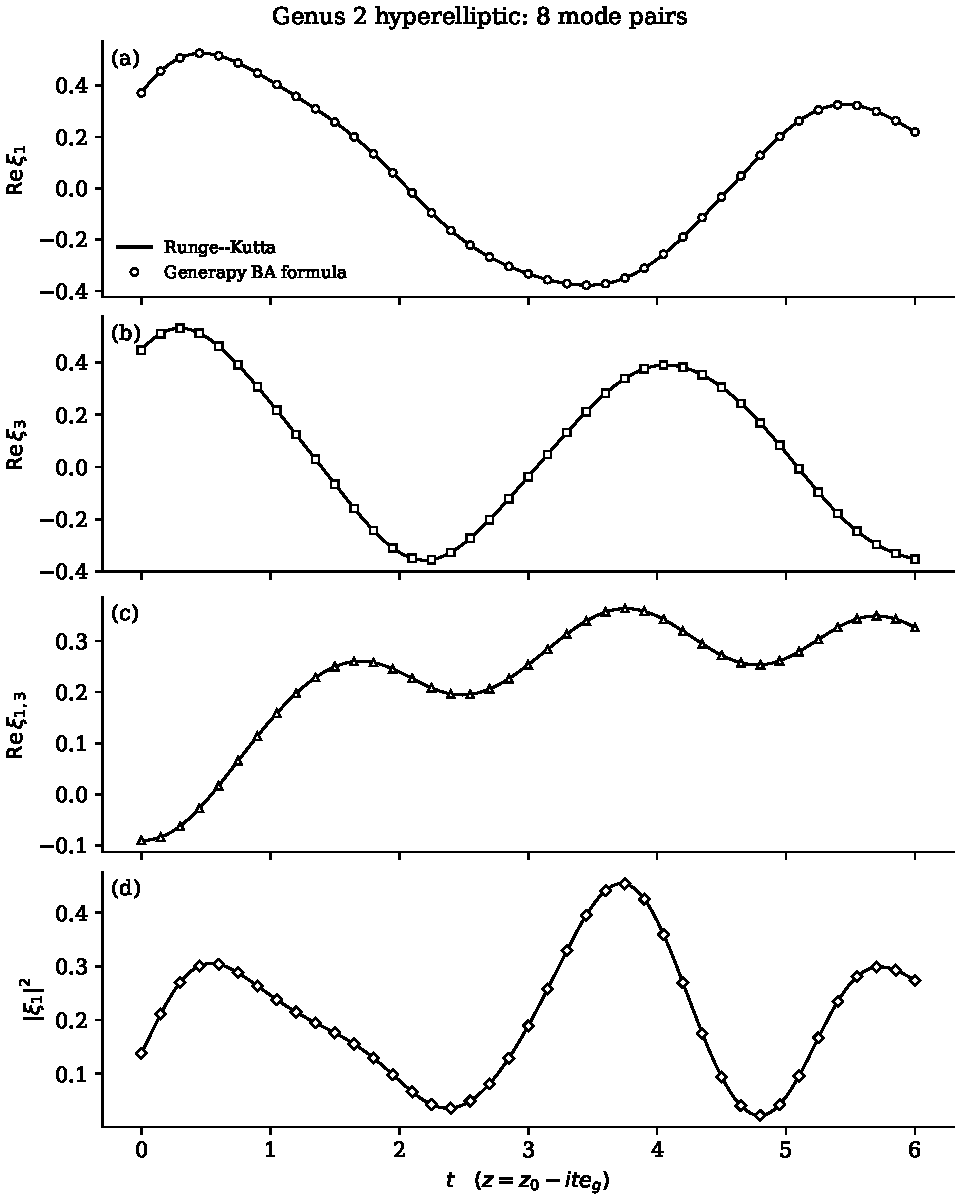
\includegraphics[width=\textwidth,height=0.82\textheight,keepaspectratio]
 {figures/hyperelliptic_sigma_ba.pdf}
 \caption{Genus-two hyperelliptic realization on
 \cref{eq:numeric-hyperelliptic-curve}. The panels show
 $\operatorname{Re}\xi_1$, $\operatorname{Re}\xi_3$,
 $\operatorname{Re}\xi_{1,3}$ and
 $|\xi_1|^2$.
 Open markers are direct Generapy BA evaluations; solid black lines
 are independent Runge--Kutta solutions of the canonical equations
 generated by $H_0$ with brackets $-i$, and $z=z_0-it e_2$.}
 \label{fig:numeric-hyperelliptic}
\end{figure}
\begin{figure}[p]
 \centering
 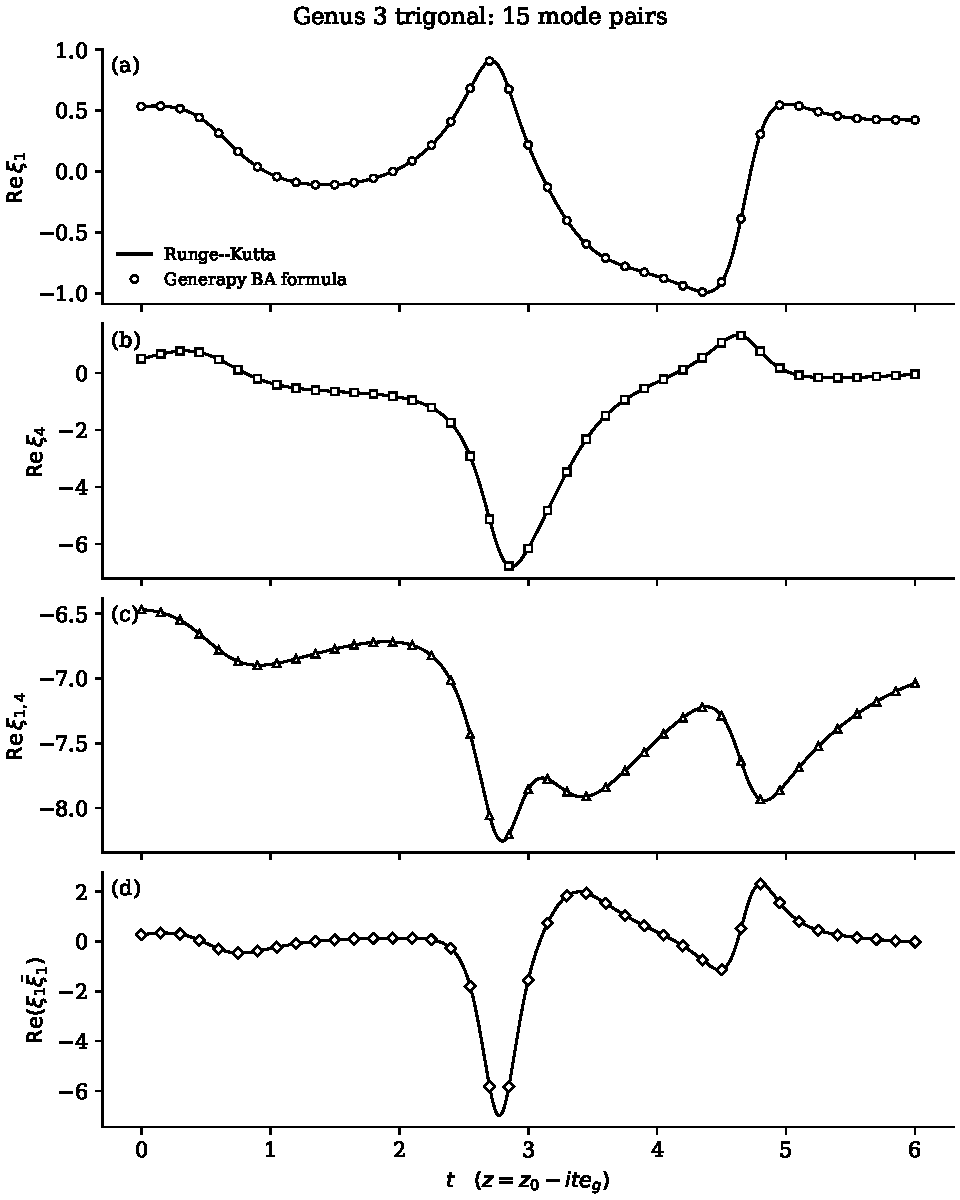
\includegraphics[width=\textwidth,height=0.82\textheight,keepaspectratio]
 {figures/trigonal_sigma_ba.pdf}
 \caption{Genus-three trigonal realization on
 \cref{eq:numeric-trigonal-curve}. The panels show
 $\operatorname{Re}\xi_1$, $\operatorname{Re}\xi_4$,
 $\operatorname{Re}\xi_{1,4}$ and
 $\operatorname{Re}(\xi_1\bar{\xi}_1)$.
 Open markers are direct Generapy BA evaluations; solid black lines
 are independent Runge--Kutta solutions of the canonical equations
 generated by $H_0$ with brackets $-i$, and $z=z_0-it e_3$.}
 \label{fig:numeric-trigonal}
\end{figure}
\begin{figure}[p]
 \centering
 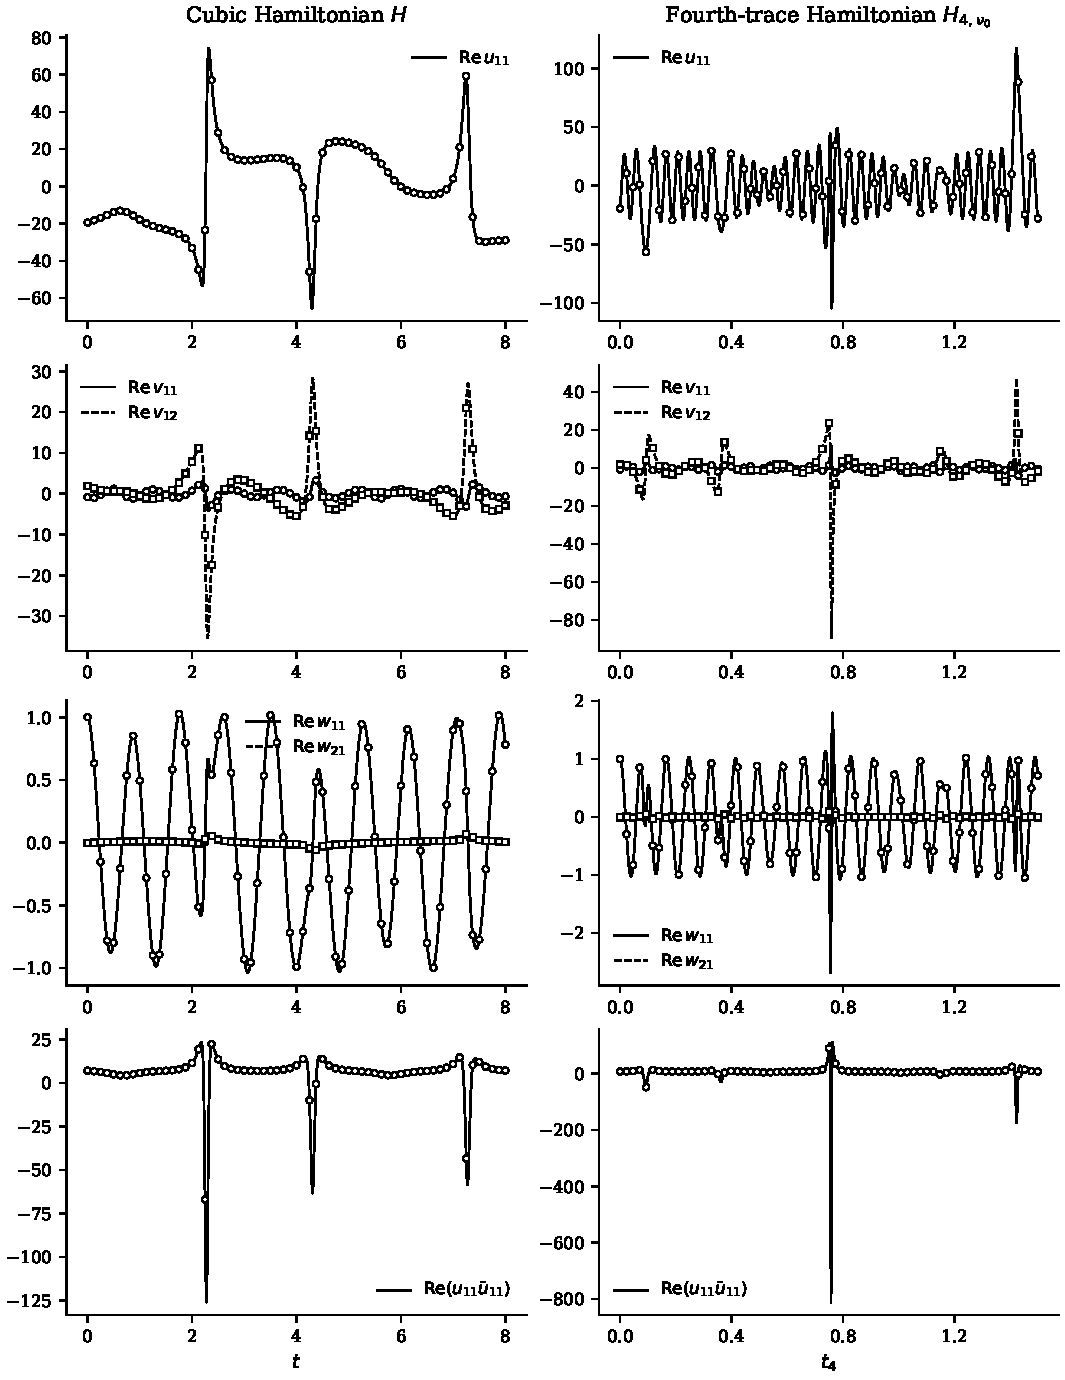
\includegraphics[width=\textwidth,height=0.82\textheight,keepaspectratio]
 {figures/multipoint_genus2_ba.pdf}
 \caption{Genus-two realization with $L=M=N=2$. Left: the cubic
 Hamiltonian $H$; right: the commuting fourth-trace Hamiltonian
 $H_{4,\nu_0}$, with $\nu_0=0.17$. Each column uses the same initial modes. The panels
 show $\operatorname{Re}u_{11}$, the two puncture-indexed modes
 $\operatorname{Re}v_{11}$ and $\operatorname{Re}v_{12}$,
 $\operatorname{Re}w_{11}$ and $\operatorname{Re}w_{21}$, and
 $\operatorname{Re}(u_{11}\bar u_{11})$.
 Open circles and squares are direct Generapy-based BA evaluations;
 solid and dashed black lines are independent RK4 trajectories.
 The barred modes are independent Hamiltonian partners.}
 \label{fig:numeric-multipoint-genus2}
\end{figure}
\clearpage
